\scanpage{12}
\uline{Frobéniuseries.}

On désigne par $(\mathrm{Sch})_p$ \inserted{$=(\mathrm{Sch})_{/\operatorname{Spec}(\mathbb Z/p\mathbb Z)}$} la sous catégorie pleine des $(\mathrm{Sch})$
formée des préschémas de car. $p$, et tous les préschémas
envisagés sont de car. $p$.

On définit un hom fonctoriel en $X$
\[
\operatorname{Frob}(X):X\longrightarrow X
\]
\margin{\figure{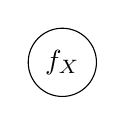
\begin{tikzpicture}\node[draw,circle] {$f_X$};\end{tikzpicture}}}
[\uline{Frobenius absolu}] par la condition d'être l'identité
sur les espaces topologiques, et $f\mapsto f^p$ sur les
fonctions.

Soit $S$ fixé. Pour tout $X$ sur $S$, on a donc
un carré commutatif
\diagram{\begin{tikzcd}
X \arrow[r,"{\operatorname{Frob}(X)}"] \arrow[d,"f"'] & X \arrow[d,"f"]\\
S \arrow[r,"{\operatorname{Frob}(S)}"'] & S
\end{tikzcd}}
\margin{\diagram{\begin{tikzcd}
X \arrow[r,"{\mathrm{Fr}_{X/S}}"] & X^{(p/S)}
\end{tikzcd}}}
\margin{Changer les flèches horizontales \unsure{de direction}}
(où $f$ est le morphisme structural). \deleted{Ainsi}, Posons
\[
\deleted{\unsure{F}}P_S(X)=X\times_S(S,\operatorname{Frob}(S)):
\]
\margin{\figure{\begin{tikzpicture}
\node[draw,ellipse] {$X^{(p/S)}$ ou $X^{(p/f)}$ ou $X^{(p)}$};
\node[anchor=north west] at (-2.1,-.35) {$(X/S)^{(p)}$};
\end{tikzpicture}}}
$\unsure{p_S|P_S}(X)$ est un foncteur
\[
P_S:(\mathrm{Sch})_{/S}\longrightarrow(\mathrm{Sch})_{/S}
\]
\margin{dire que $X\longrightarrow P_S(X)$ est un \uline{homéomorphisme}\deleted{\unsure{étale}} \uline{universel}.}
qui étant un foncteur de changement de base, en
a toutes les propriétés [commute aux
$\varprojlim$, aux sommes, transforme type fini
\mspage{11}
